\documentclass[tikz,border=4pt]{standalone}
\usepackage{amsmath}
\begin{document}
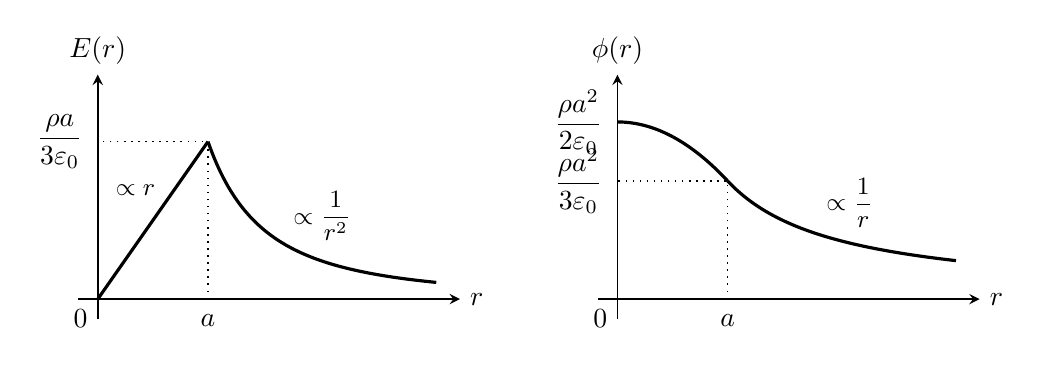
\begin{tikzpicture}[>=stealth, thick, scale=1.0]
  % Left panel: E(r)
  \begin{scope}[xshift=0cm]
    \draw[->, line width=0.65pt] (-0.25, 0) -- (4.6, 0) node[right] {$r$};
    \draw[->, line width=0.65pt] (0, -0.25) -- (0, 2.85) node[above] {$E(r)$};
    \node[below left] at (0, 0) {$0$};

    % a at x = 1.4, E(a) at y = 2.0
    \draw[dotted, line width=0.55pt] (1.4, 0) -- (1.4, 2.0) -- (0, 2.0);
    \node[below] at (1.4, -0.06) {$a$};
    \node[left] at (-0.06, 2.0) {$\dfrac{\rho a}{3\varepsilon_0}$};

    % Linear inside, 1/r^2 outside
    \draw[line width=1.15pt] (0, 0) -- (1.4, 2.0);
    \draw[line width=1.15pt, domain=1.4:4.3, samples=80, smooth] plot (\x, {2.0 * (1.4/\x)^2});

    \node[font=\small] at (0.48, 1.38) {$\propto r$};
    \node[font=\small] at (2.85, 1.05) {$\propto \dfrac{1}{r^2}$};
  \end{scope}

  % Right panel: phi(r)
  \begin{scope}[xshift=6.6cm]
    \draw[->, line width=0.65pt] (-0.25, 0) -- (4.6, 0) node[right] {$r$};
    \draw[->, line width=0.65pt] (0, -0.25) -- (0, 2.85) node[above] {$\phi(r)$};
    \node[below left] at (0, 0) {$0$};

    % a at x = 1.4, phi(a) = 1.5, phi(0) = 1.5 * 3/2 = 2.25
    \draw[dotted, line width=0.55pt] (1.4, 0) -- (1.4, 1.5) -- (0, 1.5);
    \node[below] at (1.4, -0.06) {$a$};
    \node[left] at (-0.06, 1.5) {$\dfrac{\rho a^2}{3\varepsilon_0}$};
    \node[left] at (-0.06, 2.25) {$\dfrac{\rho a^2}{2\varepsilon_0}$};

    % Parabolic inside: 2.25 - 0.75*(x/1.4)^2, 1/r outside: 1.5*(1.4/x)
    \draw[line width=1.15pt, domain=0:1.4, samples=50, smooth] plot (\x, {2.25 - 0.75*(\x/1.4)^2});
    \draw[line width=1.15pt, domain=1.4:4.3, samples=80, smooth] plot (\x, {1.5 * (1.4/\x)});

    \node[font=\small] at (2.95, 1.22) {$\propto \dfrac{1}{r}$};
  \end{scope}
\end{tikzpicture}
\end{document}
